\documentclass{article}
\usepackage[utf8]{inputenc}
\usepackage[T1]{fontenc}
\usepackage{geometry}
\geometry{
    a4paper,
    left=2.5cm,
    right=2.5cm,
    top=2.5cm,
    bottom=2.5cm
}
\usepackage{graphicx}
\usepackage{float}
\usepackage{hyperref}
\usepackage[english]{babel}
\usepackage{amsmath}
\usepackage{amssymb}
\usepackage{array}
\usepackage{booktabs}
\usepackage{caption}
\usepackage{subcaption}
\usepackage{enumitem}
\usepackage{fancyhdr}
\usepackage{titlesec}
\usepackage{url}
\usepackage{textcomp}
\usepackage{xcolor}
\usepackage{listings}
\usepackage{multirow}
\usepackage{longtable}
\usepackage{tabularx}
\usepackage{times}

% Set up page style
\pagestyle{fancy}
\fancyhf{}
\rfoot{\thepage}
\renewcommand{\headrulewidth}{0pt}

% Title formatting
\titleformat{\chapter}[display]{\normalfont\bfseries}{\chaptertitle\thechapter}{0pt}{\Huge}
\titlespacing*{\chapter}{0pt}{50pt}{40pt}

% Document info
\title{Template Document}
\author{Academic Support Agent}
\date{\today}

\begin{document}
\maketitle

\rightskip\rightmargin

\title{    \\
\textcolor{yellow}{     }}

\author{  :    }
\institute{  :            }
\date{\today}

\begin{frame}
\maketitle
\end{frame}

\begin{frame}{ }

\end{frame}



\section{       }
\subsection{ }
\begin{frame}{       }

\begin{exampleblock}{ }
                               
\end{exampleblock}

\pause

\textcolor{red}{ :} 
 
\begin{columns}

\begin{column}{0.4\linewidth}

\begin{tikzpicture}[scale=0.75]
\coordinate(A)at (0,1);
\coordinate(B)at (3,0);
\coordinate(C)at (3,2.5);
\coordinate(D)at (0,3.5);

\coordinate(E)at (2,2);
\coordinate(F)at (5,1);
\coordinate(G)at (5,3.5);
\coordinate(H)at (2,4.5);


\draw[thick](A)--(B)--(C)--(D)--cycle;
\draw[thick](B)--(F)--(G)--(H)--(D) (G)--(C);
\draw[dashed](H)--(E)--(F) (E)--(A);

\onslide<3->{\draw[red,very thick]($(H)!-0.3!(G)$)--($(G)!-0.3!(H)$)node[right]{\tiny $(D_2)$}; 
\draw[blue,very thick]($(B)!-0.3!(C)$)--($(C)!-0.3!(B)$)node[right]{\tiny $(D_1)$}; 
}

\onslide<4->{\fill[blue](G)circle(2.5pt)node[above right]{\tiny $A$};} 

\onslide<5->{\draw[dashed,blue,very thick]($(F)!-0.3!(G)$)--($(G)!-0.3!(F)$);
\draw[thick]($(G)!0.3cm!(H)$)--+(0,-0.3)--($(G)!0.3cm!(F)$);
}

\onslide<7->{\draw[OliveGreen,very thick]($(H)!-0.3!(D)$)--($(D)!-0.3!(H)$)node[above]{\tiny $(D_3)$}; }

\end{tikzpicture}

\end{column}

\begin{column}{0.5\linewidth}

\onslide<6->{

\begin{itemize}\RTListe
\item
    $A$       
$(D_1)$       $(D_2)$ 
   $(D_1)$    $(D_2)$  . 
\item
             
$(D_1)$   $(D_3)$
\end{itemize}

\vspace{2cm}

}

\end{column}

\end{columns} 
 
\end{frame}

\subsection{ }

\begin{frame}{ }
\begin{exampleblock}{}
\begin{enumerate}\rightskip\leftm
\item 
                 .

\item
         .
\end{enumerate}
\end{exampleblock}

\pause

\begin{columns}

\begin{column}{0.3\linewidth}

\begin{tikzpicture}[scale=0.75]
\coordinate(A)at (0,0);
\coordinate(B)at (3,0);
\coordinate(C)at (3,3);
\coordinate(D)at (0,3);

\coordinate(E)at (1,1);
\coordinate(F)at (4,1);
\coordinate(G)at (4,4);
\coordinate(H)at (1,4);


\draw[thick](A)--(B)--(C)--(D)--cycle;
\draw[thick](B)--(F)--(G)--(H)--(D) (G)--(C);
\draw[dashed](H)--(E)--(F) (E)--(A);

\onslide<2->{\draw[red,very thick]($(H)!-0.3!(C)$)node[above]{\tiny $(\Delta_1)$}--($(C)!-0.3!(H)$);
\draw[red,very thick,dashed]($(E)!-0.3!(B)$)node[above]{\tiny $(\Delta_2)$}--($(B)!-0.3!(E)$);
\draw[red,very thick](B)--($(B)!-0.3!(E)$);
}

\onslide<3->{\draw[blue,very thick]($(G)!-0.2!(D)$)node[above]{\tiny $(D)$}--($(D)!-0.2!(G)$);
\draw[thick](2.2,3.4)--(2.4,3.45)--(2.2,3.55);
}

\end{tikzpicture}
\end{column}

\begin{column}{0.65\linewidth}


\begin{itemize}\RTListe

\item<2->
 
 $(\Delta_1)$   $(\Delta_2)$   

\item<3-> 
  
$(D)$       $(\Delta_1)$

\item<4-> 
     
$(D)$      $(\Delta_2)$ 

\end{itemize}
\end{column}
\end{columns}

\end{frame}
\section{     }
\subsection{ }
\begin{frame}{     }
\pause
\begin{exampleblock}{ }
                                 .
\end{exampleblock}
 
\pause
 
\begin{block}{ }
                               
\end{block} 
 
\pause 
 
 \textcolor{red}{ :}
 
\begin{columns} 
\begin{column}{0.35\textwidth}
\vspace{-3mm}
\centering

\begin{tikzpicture}[scale=0.5]
\coordinate(A)at (0,0);
\coordinate(B)at (3,0);
\coordinate(C)at (3,3);
\coordinate(D)at (0,3);

\coordinate(E)at (1,1);
\coordinate(F)at (4,1);
\coordinate(G)at (4,4);
\coordinate(H)at (1,4);


\draw[thick](A)--(B)--(C)--(D)--cycle;
\draw[thick](B)--(F)--(G)--(H)--(D) (G)--(C);
\draw[dashed](H)--(E)--(F) (E)--(A);

\onslide<2->{
\foreach \i in{B,F}{\fill[red](\i)circle(2.5pt)node[right,black]{\tiny $\i$};
}
\fill[red](A)circle(2.5pt)node[left,black]{\tiny $A$};
\draw[red,very thick]($(B)!-0.2!(C)$)--($(C)!-0.3!(B)$)node[below left]{\tiny $(\Delta)$};
\draw[thick](2.7,0)--(2.7,0.3)--(3,0.3);
\draw[thick](3,0.3)--(3.2,0.55)--(3.2,0.2);
}

\onslide<6->{\foreach \i in {0.2,0.4,...,2.8} {\draw($(E)+(\i,0)$)--($(A)+(\i,0)$);}}

\end{tikzpicture}
\end{column}
\begin{column}{0.6\textwidth}
\raggedleft
\only<5->{
  $(\Delta)$           : 
$(BA)$   $(BF)$             
$(ABF)$}

\end{column}
\end{columns}

\end{frame}


\subsection{ }
\begin{frame}{ }

\begin{exampleblock}{}
\begin{enumerate}\rightskip\leftm
\item<2-> 
                 .

\item<2->
                 .

\vspace{5mm}

\item<3->
           .

\item<3->
           .

\vspace{5mm}

\item<4->
                 .

\item<4->
                 .

\end{enumerate}
\end{exampleblock}

\end{frame}



\section{   }
\subsection{ }
\begin{frame}{   }

\begin{exampleblock}{ }
                        .
\end{exampleblock}

\pause

\textcolor{red}{ }

\begin{columns}

\begin{column}{0.35\linewidth}

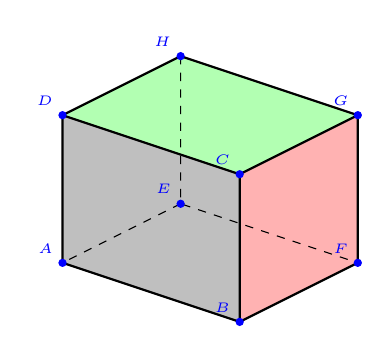
\begin{tikzpicture}[scale=0.75]
\coordinate(A)at (0,1);
\coordinate(B)at (3,0);
\coordinate(C)at (3,2.5);
\coordinate(D)at (0,3.5);

\coordinate(E)at (2,2);
\coordinate(F)at (5,1);
\coordinate(G)at (5,3.5);
\coordinate(H)at (2,4.5);


\onslide<3>{\fill[red!30](C)--(B)--(F)--(G)--cycle;
\fill[green!30](C)--(G)--(H)--(D)--cycle;
}

\onslide<4->{\fill[red!30](C)--(B)--(F)--(G)--cycle;
\fill[gray!50](A)--(B)--(C)--(D)--cycle;
}

\draw[thick](A)--(B)--(C)--(D)--cycle;
\draw[thick](B)--(F)--(G)--(H)--(D) (G)--(C);
\draw[dashed](H)--(E)--(F) (E)--(A);


\foreach \i in{A,B,C,D,E,F,G,H}{\fill[blue](\i)circle(2pt)node[above left]{\tiny $\i$};}

\end{tikzpicture}

\end{column}

\begin{column}{0.6\linewidth}

\raggedleft

\onslide<2->{
      
$ABCDEFGH$
}

\begin{itemize}\RTListe

\item<3->
  
$(BCG)$   $(DCG)$
       

 
\item<4->
             
$(BCG)$   $(ADC)$

\end{itemize}

\end{column}

\end{columns}

\end{frame}
\subsection{ }
\begin{frame}{ }
\begin{exampleblock}{}
\begin{enumerate}\rightskip\leftm

\item 
                 .

\item
	    $(P)$   $(P')$        
                      $(Q)$     
                $(P)$   $(P')$       $(Q)$.


\end{enumerate}
\end{exampleblock}
\end{frame}

\section{ }

\setbeamertemplate{enumerate item}[circle]

\begin{frame}{  47   209}
$ABCD$ 
      $AD=DC$   $AB=BC$  
$M$
  $[AC]$.
\begin{enumerate}\RTListe

\item
      $(AC)$       $(BDM)$.

\item
      $(AC)$       $(BD)$.

\end{enumerate}

\pause

\vspace{-5mm}

\begin{columns}
\begin{column}{0.27\textwidth}
\begin{tikzpicture}[scale=0.7,equal/.style={fill=red,inner sep=0pt,minimum width=2mm}]
\coordinate (D) at (0,0);
\coordinate (C) at (2.5,-1);
\coordinate (B) at (5,0);
\coordinate (A) at (2,4);
\coordinate (M) at ($(A)!0.5!(C)$);

\onslide<5->{\fill[red!20](M)--(D)--(B)--cycle;}

\draw [dashed](B)--(D);
\draw[thick](D)--(C)--(B)--(A)--cycle (A)--(C);

\foreach \i/\j in {A/above,B/right,C/below,D/left}{\fill[blue](\i)circle (2pt)node[\j]{\tiny $\i$};}

\onslide<4->{
\fill[red](M)circle(2pt)node[above right]{\tiny $M$};
\draw[red,thick](B)--(M)--(D);
\foreach \i in {A,C}{
\node[equal,rotate=5] at ($(M)!.5!(\i)$){};
}}
%
\onslide<3->{
\foreach \i in {.5,.52}{\node [equal,rotate=45] at ($ (A)!\i!(B) $) {};}
\foreach \i in {.5,.54}{\node [equal,rotate=100] at ($ (B)!\i!(C) $) {};}
\foreach \i in {.48,.5,.52}{\node [equal,rotate=-30] at ($ (A)!\i!(D) $) {};}
\foreach \i in {.47,.5,.53}{\node [equal,rotate=70] at ($ (D)!\i!(C) $) {};}
}
\end{tikzpicture}
\end{column}

\begin{column}{0.73\textwidth}

\begin{itemize}\RTListe
\item<6-| alert@6>
 
 $ABC$   $ADC$
        
  $(BM)$   $(DM)$
               .
   
        
   $(AC)$         
                 
  $(BDM)$.

\item<7-| alert@7>
  
$(AC)$       
$(BDM)$                     
$(BD)$.

\end{itemize}

\onslide<8->{}

\end{column}

\end{columns}

\end{frame}
\end{document}